\documentclass{article}

\usepackage{graphicx} % Required for inserting images
\usepackage{amsthm}
\usepackage{amssymb}
\usepackage{titlesec}
\usepackage{blindtext}
\usepackage{mathtools}
\usepackage{listings}
\usepackage{amsmath}

\let\OLDthebibliography\thebibliography
\renewcommand\thebibliography[1]{
  \OLDthebibliography{#1}
  \setlength{\parskip}{0pt}
  \setlength{\itemsep}{0pt plus 0.3ex}
}

\usepackage{titlesec}
\titlespacing*{\subsection}{0pt}{0.05\baselineskip}{0.05\baselineskip}

\usepackage{titlesec}
\titlespacing*{\section}{0pt}{0.005\baselineskip}{0.1\baselineskip}

\setcounter{secnumdepth}{0}


\title{On Minkowski Spaces And Other Problems In Linear Algebra}
\author{Ben Lowe, Caleb Loveridge, Chloe Godwin, \\ Rebecca Grimshaw, Moritz Hartmann }
\date{November 2023}

\begin{document}

\maketitle

\tableofcontents

\break 

\section{Part A}
First, we have that any orthogonal sequence of vectors is linearly independent. This means if we have a sequence of vectors $v_i$, then for all $i,j$ st $i \neq j$ then $<v_i|w_j> = 0$ then we know that for $\sum_i \alpha_i v_i = 0$ implies that all $\alpha_i$ is linear independence.

Construct, $\sum_i \alpha_i v_i = 0$ then for orthogonal vectors we apply the inner product of the sum with $v_j$ for some j and see $0 = <v_k | \sum_i \alpha_i v_i> = \sum_i \alpha_i <v_j|v_i>$ by linearity. Then we evaluate the inner products and see that all become zero except for when $j=i$ which by positive definiteness we know is positive so $\alpha_i <v_i|v_i> = 0$ means that $\alpha_i$ must be zero hence the sequence is linearly independent. 

\subsection*{Part A Question 2}
Spectral decomposition is the special case of the change of bases where the change of basis matrices is the orthogonal matrix given by the Eigen column vectors of the matrix A  multiplied to a diagonal matrix of the A's eigenvalues. This means that if we have the spectral decomposition, $A = P^T D P$ where $A$ is symmetric, $P$ is orthogonal and $D$ is diagonal the we can write this as the change of basis $ _B[A]_B = _B[Id]_C[D]_C[Id]_B$ where the basis is the eigenvectors of A.

\subsection*{Part A Question 3}
when a group member works in a kitchen it is important to work out the individual costs of ingredients when ordering in bulk. For each order we can write this as the row of a matrix. The solution set gives the unit costs of ingredients. This is then used to find the cost of individual dishes.



Let $x_1 = $Price of Carrot

Let $x_2 = $Price of Pepper

Let $x_3 = $Price of Tomato

On different orders by the kitchen, various numbers of each ingredient are ordered, where the RHS equals the order cost and the coefficients the quantity of ingredients.

Order 1: $100x_1 + 40x_2 + 250x_3 = 71.5$

Order 2: $80x_1 + 200x_2 + 100x_3 = 101$

Order 3: $300x_1 +50x_2 + 120x_3 = 95.5$

In form $Ax=b$.

\begin{equation*}
     \begin{bmatrix}
         100 & 40 & 250 \\ 80 & 200 & 100 \\ 300 & 50 & 120
     \end{bmatrix}
     \begin{bmatrix}
         x_1 \\ x_2 \\ x_3
     \end{bmatrix}
     =
     \begin{bmatrix}
         71.5 \\ 101 \\ 95.5
     \end{bmatrix}
\end{equation*}

Solve system by putting A in augmented matrix and row reducing:

\begin{equation*}
    \Bigg[
    \begin{matrix}
         100 & 40 & 250 \\ 80 & 200 & 100 \\ 300 & 50 & 120
     \end{matrix}
     \Bigg|
     \begin{matrix}
         71.50 \\ 101.00 \\ 95.50
     \end{matrix}
     \Bigg]
     \mapsto
     \Bigg[
     \begin{matrix}
         1 &0&0\\ 0&1&0\\0&0&1
     \end{matrix}
     \Bigg{|}
     \begin{matrix}
         0.20 \\ 0.35 \\ 0.15
     \end{matrix}
     \Bigg]
\end{equation*}

This provides the result $x_1 = 0.2, x_2 = 0.35, x_3 = 0.15$, such that.

\begin{equation*}
    x =
    \begin{bmatrix}
        0.2 \\0.35 \\0.15
    \end{bmatrix}
\end{equation*}

And,
\begin{equation*}
     \begin{bmatrix}
         100 & 40 & 250 \\ 80 & 200 & 100 \\ 300 & 50 & 120
     \end{bmatrix}
     \begin{bmatrix}
         x_1 \\ x_2 \\ x_3
     \end{bmatrix}
     =
     \begin{bmatrix}
         71.5 \\ 101 \\ 95.5
     \end{bmatrix}
\end{equation*}

The solution set of x provides the individual price of carrots, peppers and tomatoes respectively.





\subsection*{Part A Question 4}
This week we met up in person all at the same time, as well as getting it done earlier to give us more time to check offer the work.
As a group we have reflected on the feedback that was given from the last project leading to us changing how we complete part A and allowing us to ensure we complete the tasks accurately.

We haven't been able to find out what went wrong in our answer to part C in the first project. Also, during the last project we were not able to all meet up at the same time sue to scheduling issues.
The in-person meetups have been productive as we've managed to complete all of part A together.
We've had efficient communication channels which has allowed us to plan in-person meetings faster compared to the last group project.

\break
\section{Part B}

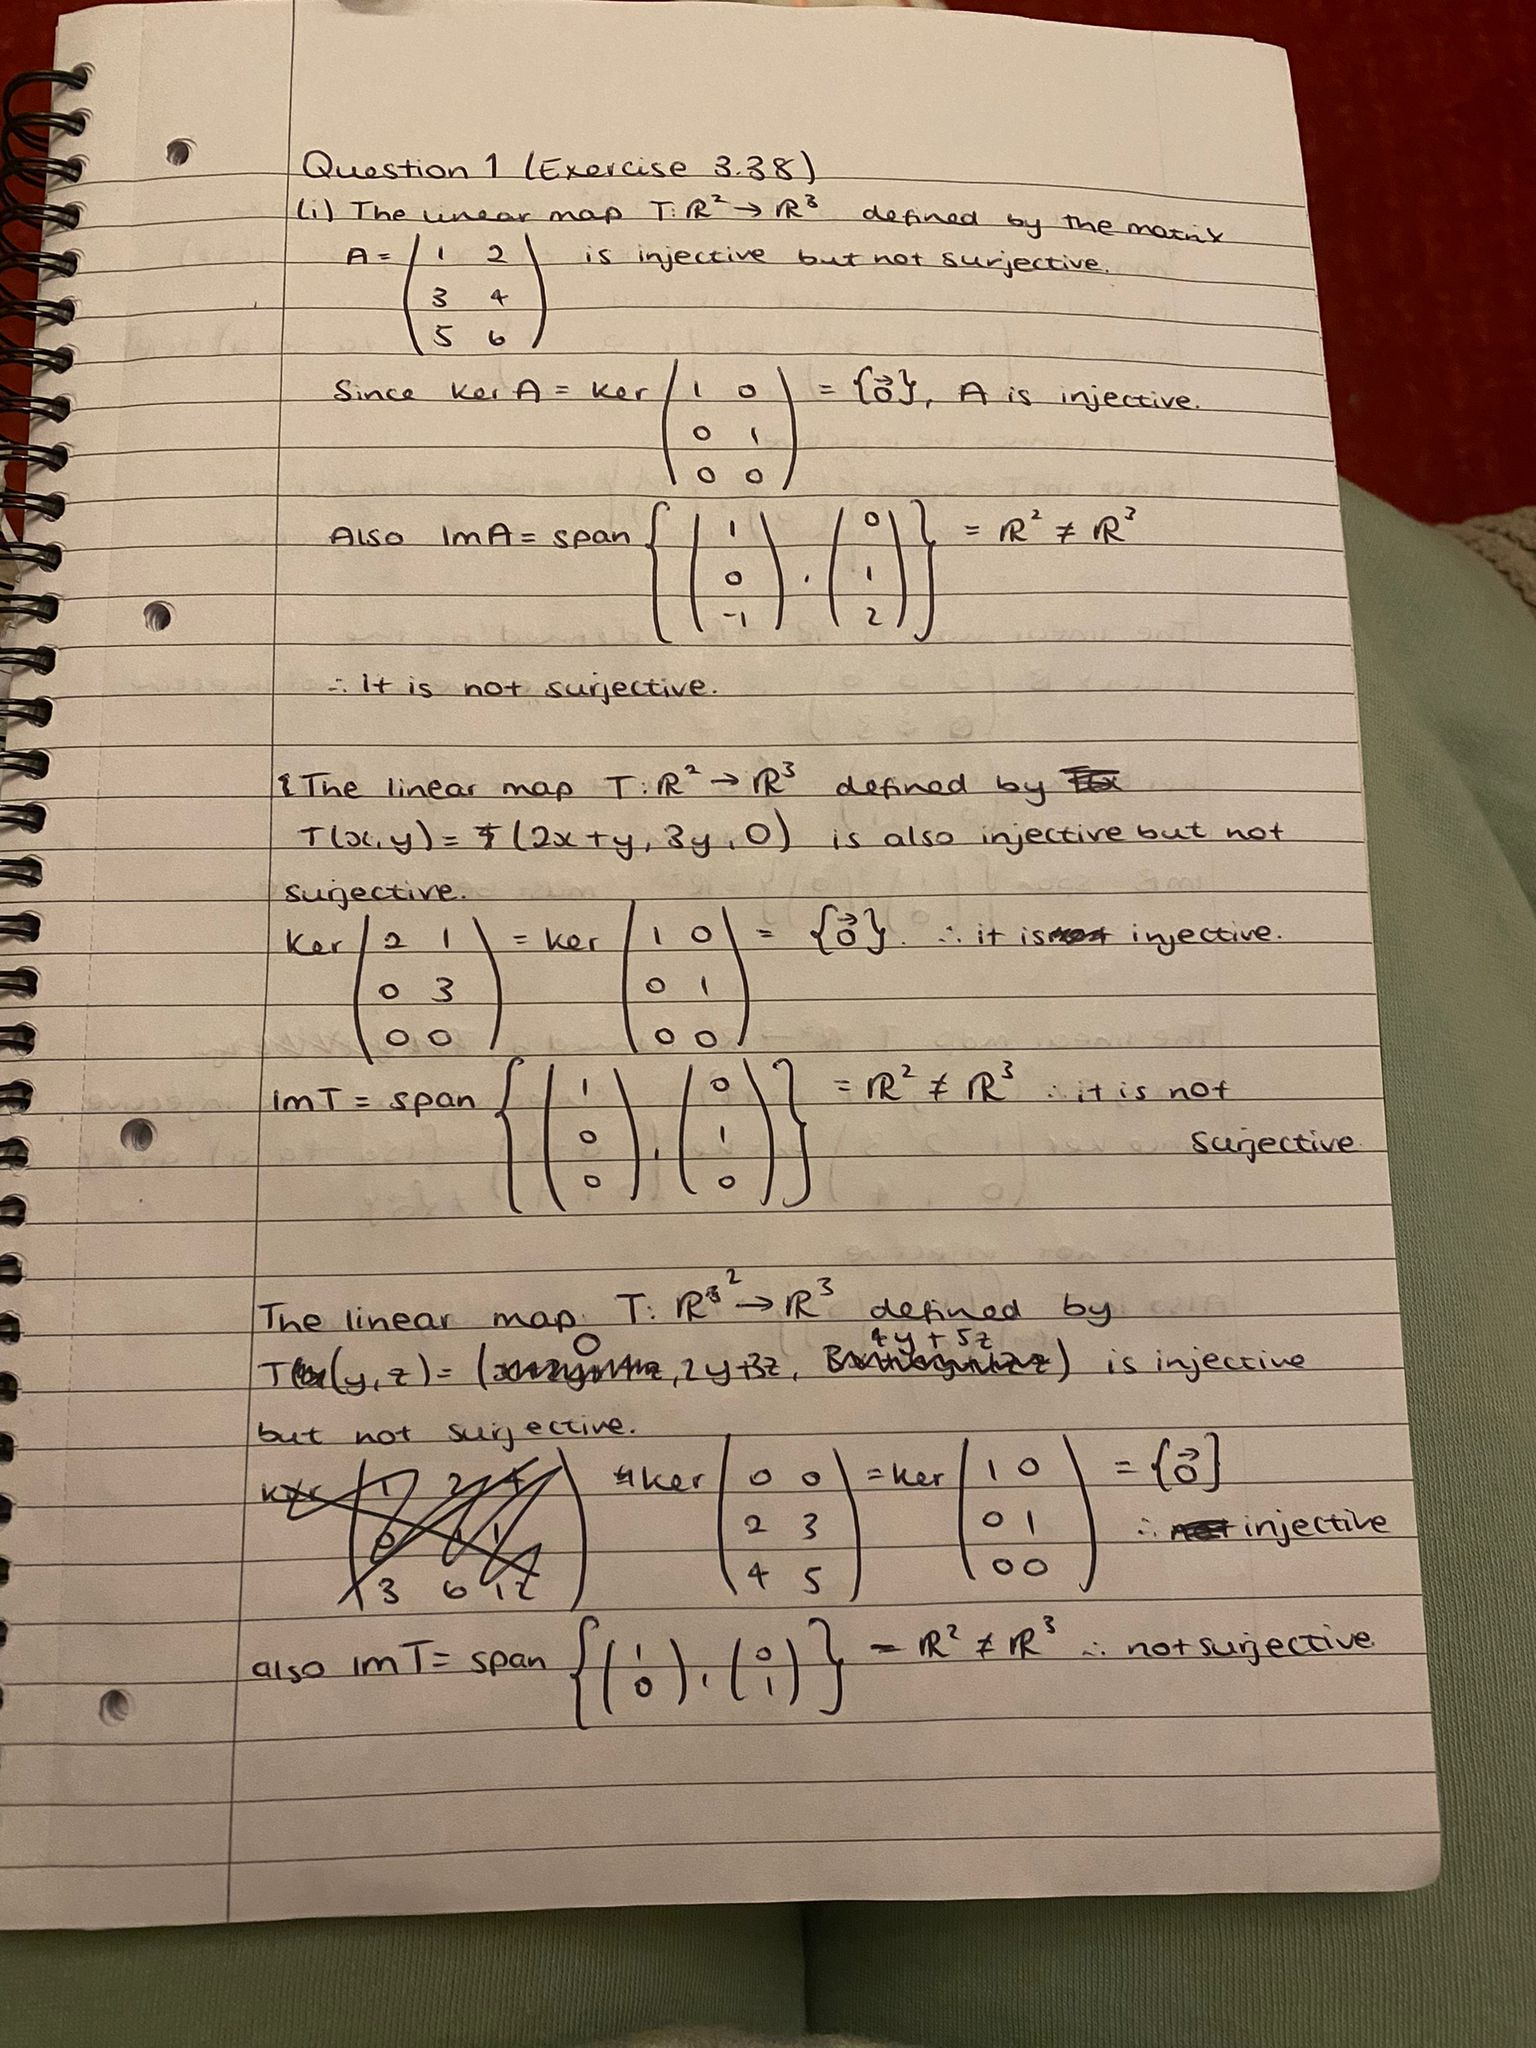
\includegraphics[scale = 0.2]{IMG-20231126-WA0002.jpg}

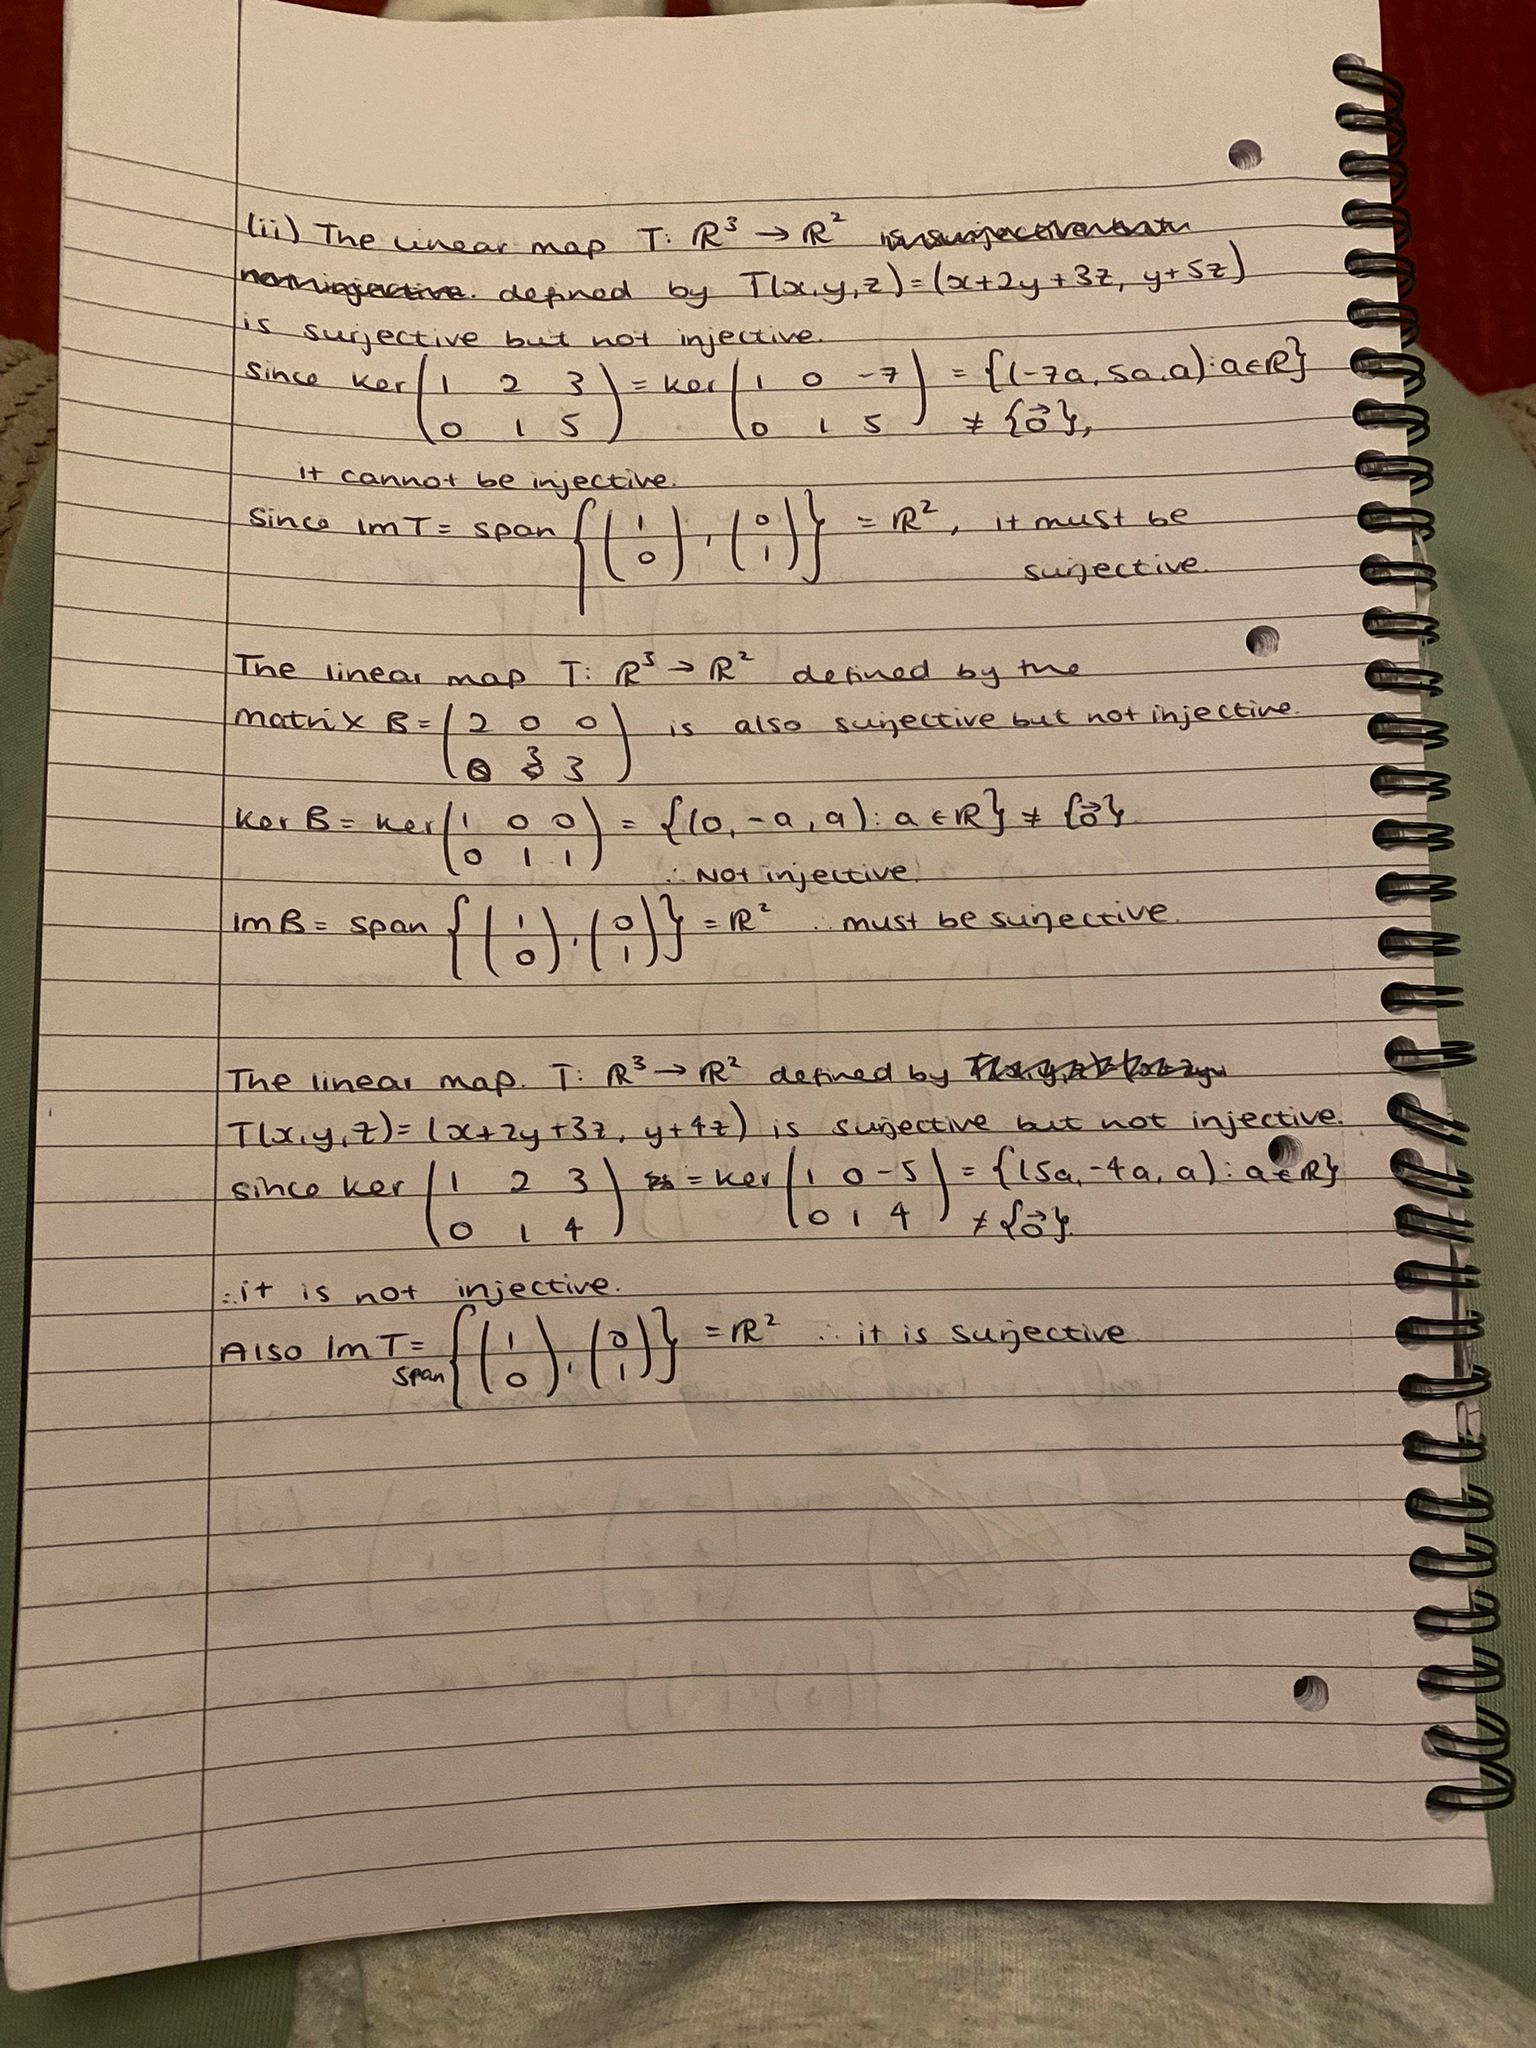
\includegraphics[scale = 0.2]{IMG-20231126-WA0005.jpg}

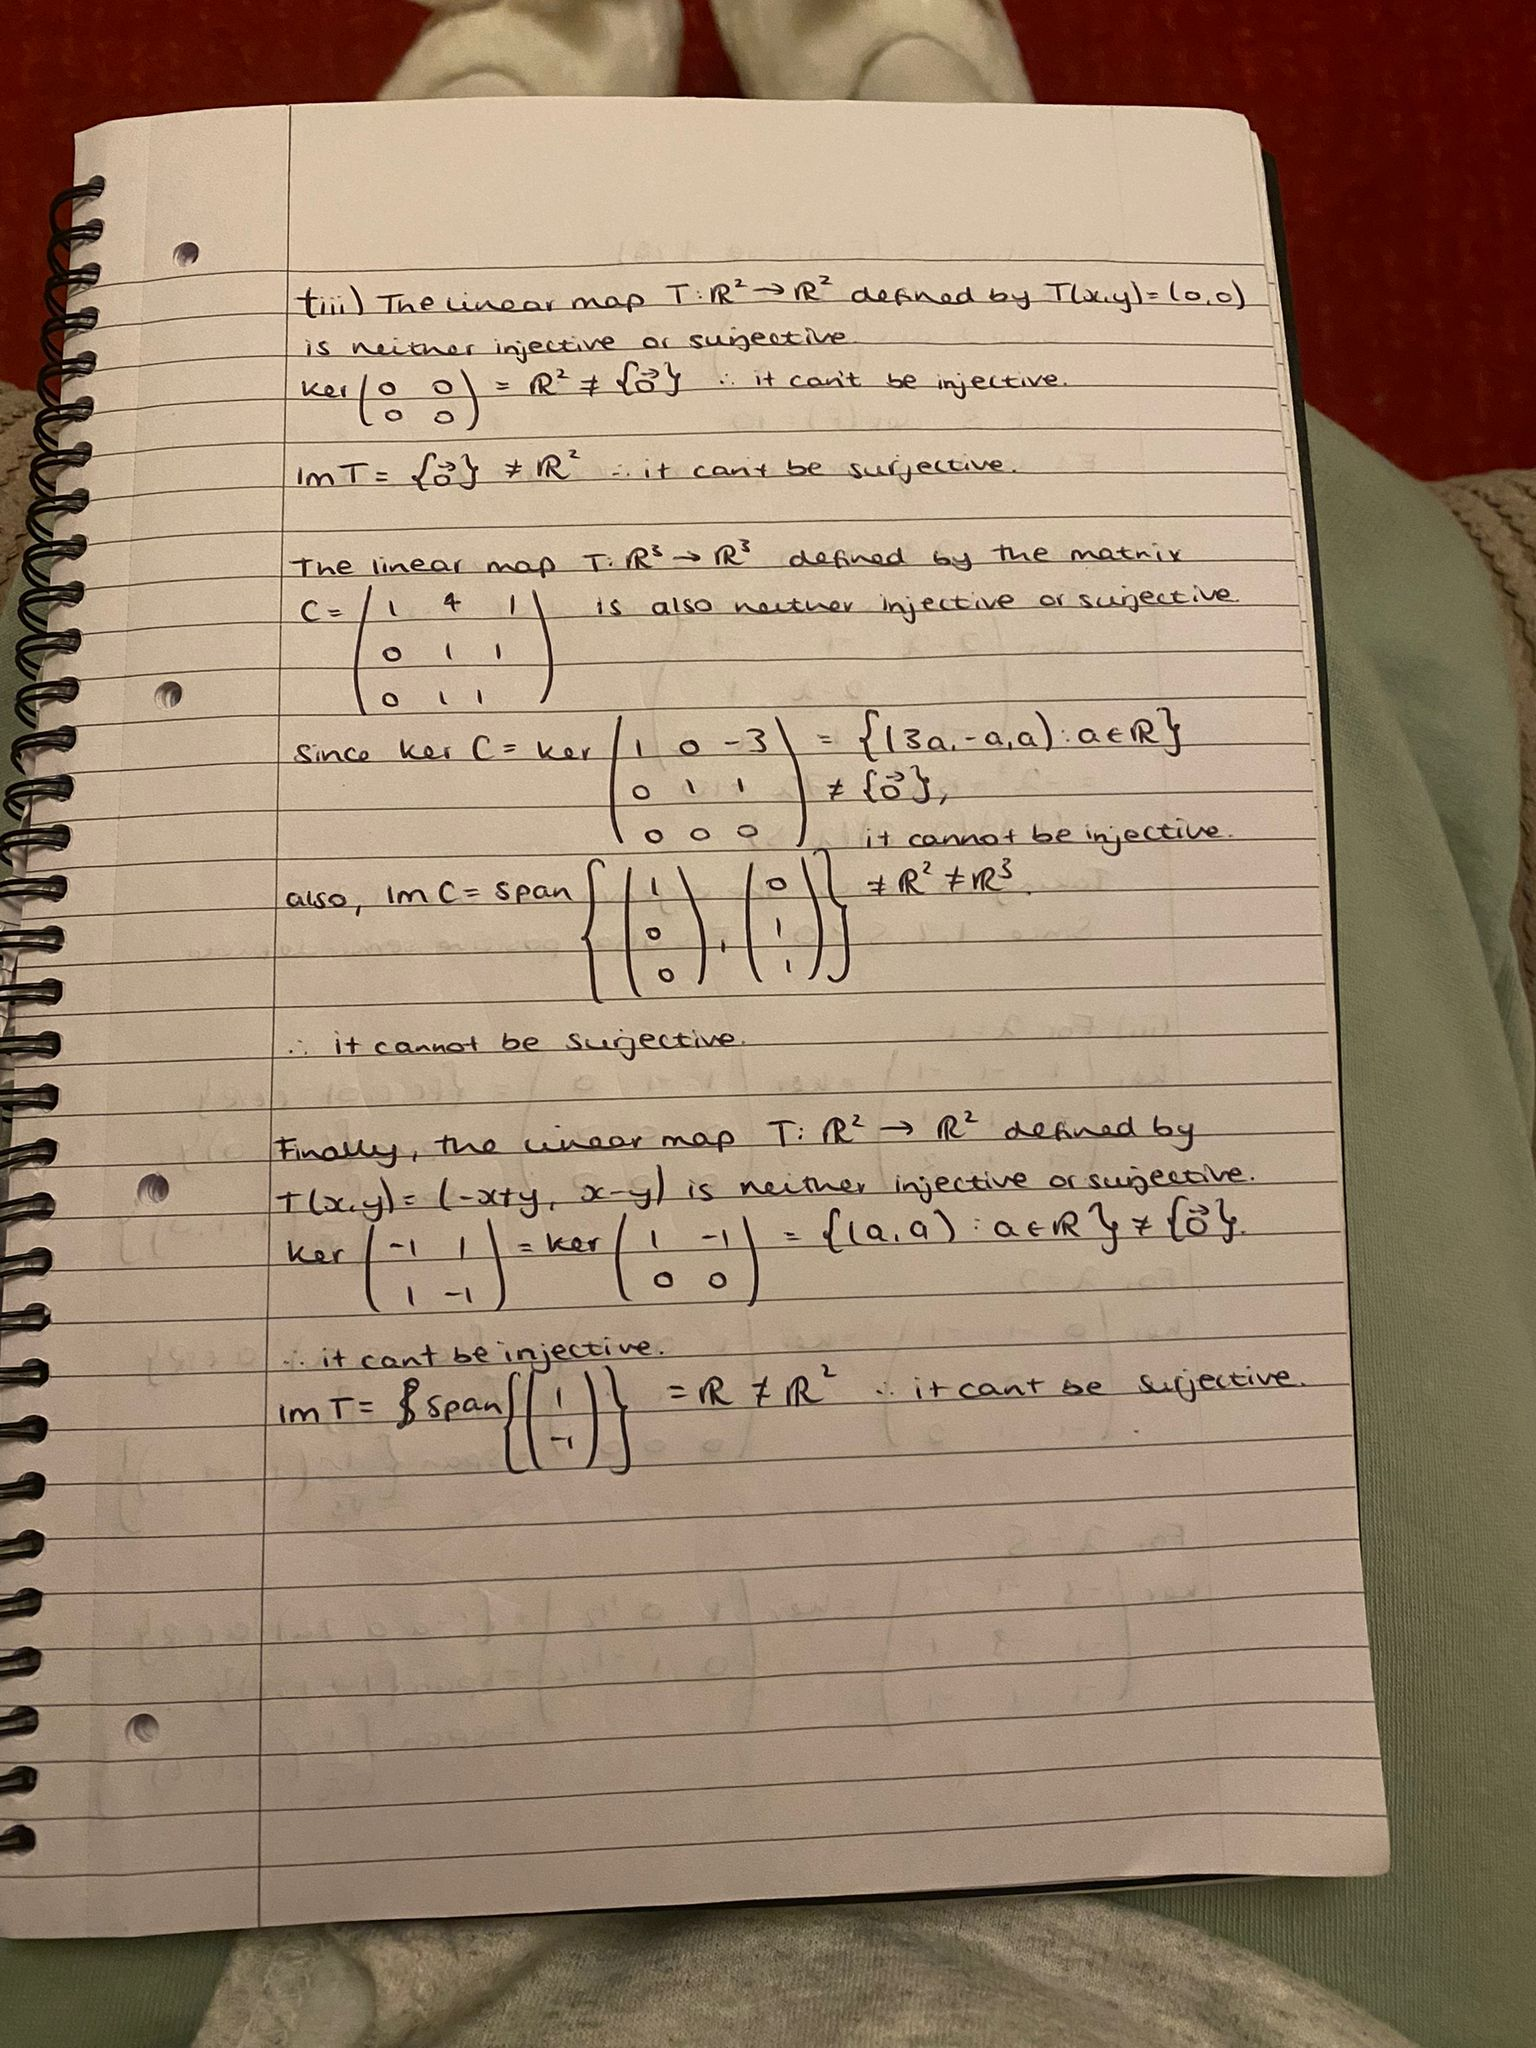
\includegraphics[scale = 0.2]{IMG-20231126-WA0004.jpg}



\break








\subsection*{Part B Question 2}
(i)
Verify that $ \mathcal{B}=((3,-1),(-2,1)) $ consists of eigenvectors of $A := \begin{bmatrix}
    -5 & -18 \\ 3 & 10
\end{bmatrix}$

In order to find the eigenvectors of A, first we must find the eigenvalues $\lambda$ by finding the roots of the characteristic polynomial of A

\begin{align*}
    \det(A-\lambda I) =& 0 \\
    \det \begin{bmatrix}
        -5-\lambda & -18 \\ 3 & 10 - \lambda
    \end{bmatrix}
    =& 0
\end{align*}

Simplifying we get

\begin{equation*}
    (\lambda - 1) (\lambda - 4)
\end{equation*}

Therefore, the eigenvalues are $ \lambda = 1, \lambda = 4 $
Then to find the eigenvectors $ V $, we find the kernel of $ (A – \lambda I) $, substituting in the eigenvalues. 
Firstly, for $ \lambda = 1 $

\begin{align*}
    v_{1} 
    &= \ker\begin{bmatrix}
        -5-5 & -18 \\ 3 & 10-1
    \end{bmatrix}\\
    &= \ker \begin{bmatrix}
        -6 & -18 \\ 3 & 9
    \end{bmatrix}\\
    &= \begin{bmatrix}
        1 & 3 \\ 0 & 0
    \end{bmatrix}\\
    &= \text{span}  
    \begin{pmatrix}
        3 \\ -1
    \end{pmatrix}
\end{align*}

Then for $ \lambda = 4 $

\begin{align*}
    v_{4} &= \\
    &= \ker \begin{bmatrix}
        -5-4 & -18 \\ 3 & 10-4
    \end{bmatrix}
    &= \ker \begin{bmatrix}
        -9 & -18 \\ 3 & 6
    \end{bmatrix} \\
    &=
    \ker\begin{bmatrix}
        1 & 2 \\ 0 & 0
    \end{bmatrix} \\
    &= \text{span} \begin{pmatrix}
        -2 \\ 1
    \end{pmatrix}
\end{align*}

Hence, we have shown that $ \mathcal{B}=((3,-1),(-2,1)) $ consists of eigenvectors of A

(ii.)
Verify, by matrix multiplication, that $D := P^{-1} A P$ is a diagonal matrix.
Firstly we must calculate $ P^-1  $

\begin{align*}
    P &= \begin{bmatrix}
        3 & -2 \\ -1 & 1
    \end{bmatrix} \\
    P^{-1} &=
    \begin{pmatrix}
        1 & 2 \\ 1 & 3
    \end{pmatrix}
\end{align*}

Now we can verify by matrix multiplication 

\begin{align*}
    D &= 
    \begin{bmatrix}
        1 & 2 \\ 1 & 3
    \end{bmatrix}
    \begin{bmatrix}
        -5 & -18\\ 3 & 10
    \end{bmatrix}
    \begin{bmatrix}
        3 & -2 \\ -1 & 1
    \end{bmatrix} \\
    &= 
    \begin{bmatrix}
        1 & 2 \\ 1 & 3
    \end{bmatrix}
    \begin{bmatrix}
        3 & -8 \\ -1 & 4
    \end{bmatrix} \\
    &=\begin{bmatrix}
        1 & 0 \\ 0 & 4
    \end{bmatrix}
\end{align*}

Hence, D is a diagonal matrix

(iii.)
Verify, by matrix multiplication, that $A = P D P^{-1}$

\begin{align*}
    A &=
    \begin{bmatrix}
        3 & -2 \\ -1 & 1
    \end{bmatrix}
    \begin{bmatrix}
        1 & 0 \\ 0 & 4
    \end{bmatrix}
    \begin{bmatrix}
        1 & 2 \\ 1 & 3
    \end{bmatrix} \\
    &=
    \begin{bmatrix}
        3 & -2 \\ -1 & 1
    \end{bmatrix}
    \begin{bmatrix}
        1 & 7 \\ 4 & 12
    \end{bmatrix} \\
    &=
    \begin{bmatrix}
        -5 & -18 \\ 3 & 10
    \end{bmatrix}
\end{align*}



\subsection*{Part B Question 3}
3.55) “Prove that similar matrices always have the same eigenvalues”.

Two square matrices $A$ and $B$ are said to be similar if there exists an invertible matrix P such that $A=P^{-1}BP$.

The characteristic polynomial of $A$, denoted $CA(\lambda)$, is equal to the determinant of $A$ minus $\lambda$ times the identity matrix $CA(\lambda ) = \det(A- \lambda I_n).

The roots of the characteristic polynomial are equal to the eigenvalues, so to prove that $A$ and $B$ have the same eigenvalues, you must prove that their characteristic polynomials are equal $ CA(\lambda )= CB(\lambda ) $.

To prove the characteristic polynomials of $A$ and $B$ are equal, substitute $A=P^{-1}BP$ into the equation for the characteristic polynomial of A, resulting in $CA(\lambda )=\det(P^{-1}BP - \lambda I_n)$.

This can then be re-written as $\det(P^{-1}(B- \lambda I_n)P)$, where you can then apply the multiplicative property of determinants to obtain $\det(P^{-1})\det(B- \lambda I_n)\det(P)$.

Since the product of the determinant of an invertible matrix and the determinant of its inverse is equal to $1$, we then obtain that $CA(\lambda )= \det(B- \lambda I_n)= CB(\lambda )$, thus showing that the similar matrices A and B have equal characteristic polynomials, and therefore the same eigenvalues.


Mistake in ChatGPT response:

The ChatGPT response states that $\det(B)\det(I_n-\lambda P^{-1})=\det(B-\lambda I_n)$, which is incorrect. 

$\det(B) \det(I_n-\lambda P^{-1}) = \det(B-\lambda BP^{-1})$ 
These aren’t equivalent since $BP^{-1}$ is not equal to the identity matrix.


\subsection{Part B Question 4}
We must prove that there is no matrix \(B \in M_2(\mathbb{C})\) 
such that \(B^2 = 
\begin{bmatrix}
    0 & 1 \\
    0 & 0 \\
\end{bmatrix}\).

From the lecture notes, we know that a matrix \(A \in M_2(\mathbb{C})\) 
only has a square root, such that \(A = B^2\), if \(A\) is positive semi-definite.

In our case, we let \(A = B^2 = 
\begin{bmatrix}
    0 & 1 \\
    0 & 0 \\
\end{bmatrix}\).

To determine if this particular matrix is positive semi-definite, we need to check if its eigenvalues are strictly positive.

For finding the eigenvalues of a matrix, we apply the formula 
\[
\det(A - \lambda I) = 0.
\]

So we get that
\[
\det
\begin{bmatrix}
    -\lambda & 1 \\
    0 & -\lambda \\
\end{bmatrix}
= 0
\]
which gives us the equation \(0 = (-\lambda)(-\lambda)\).


Thus, the eigenvalues of \(A\) are just 0, and thus our matrix \(A\) has no square root since it is not positive semi-definite.
So there exists no matrix \(B \in M_2(\mathbb{C})\) 
such that \(B^2 = 
\begin{bmatrix}
    0 & 1 \\
    0 & 0 \\
\end{bmatrix}\).

\subsection{Part B Question 5}

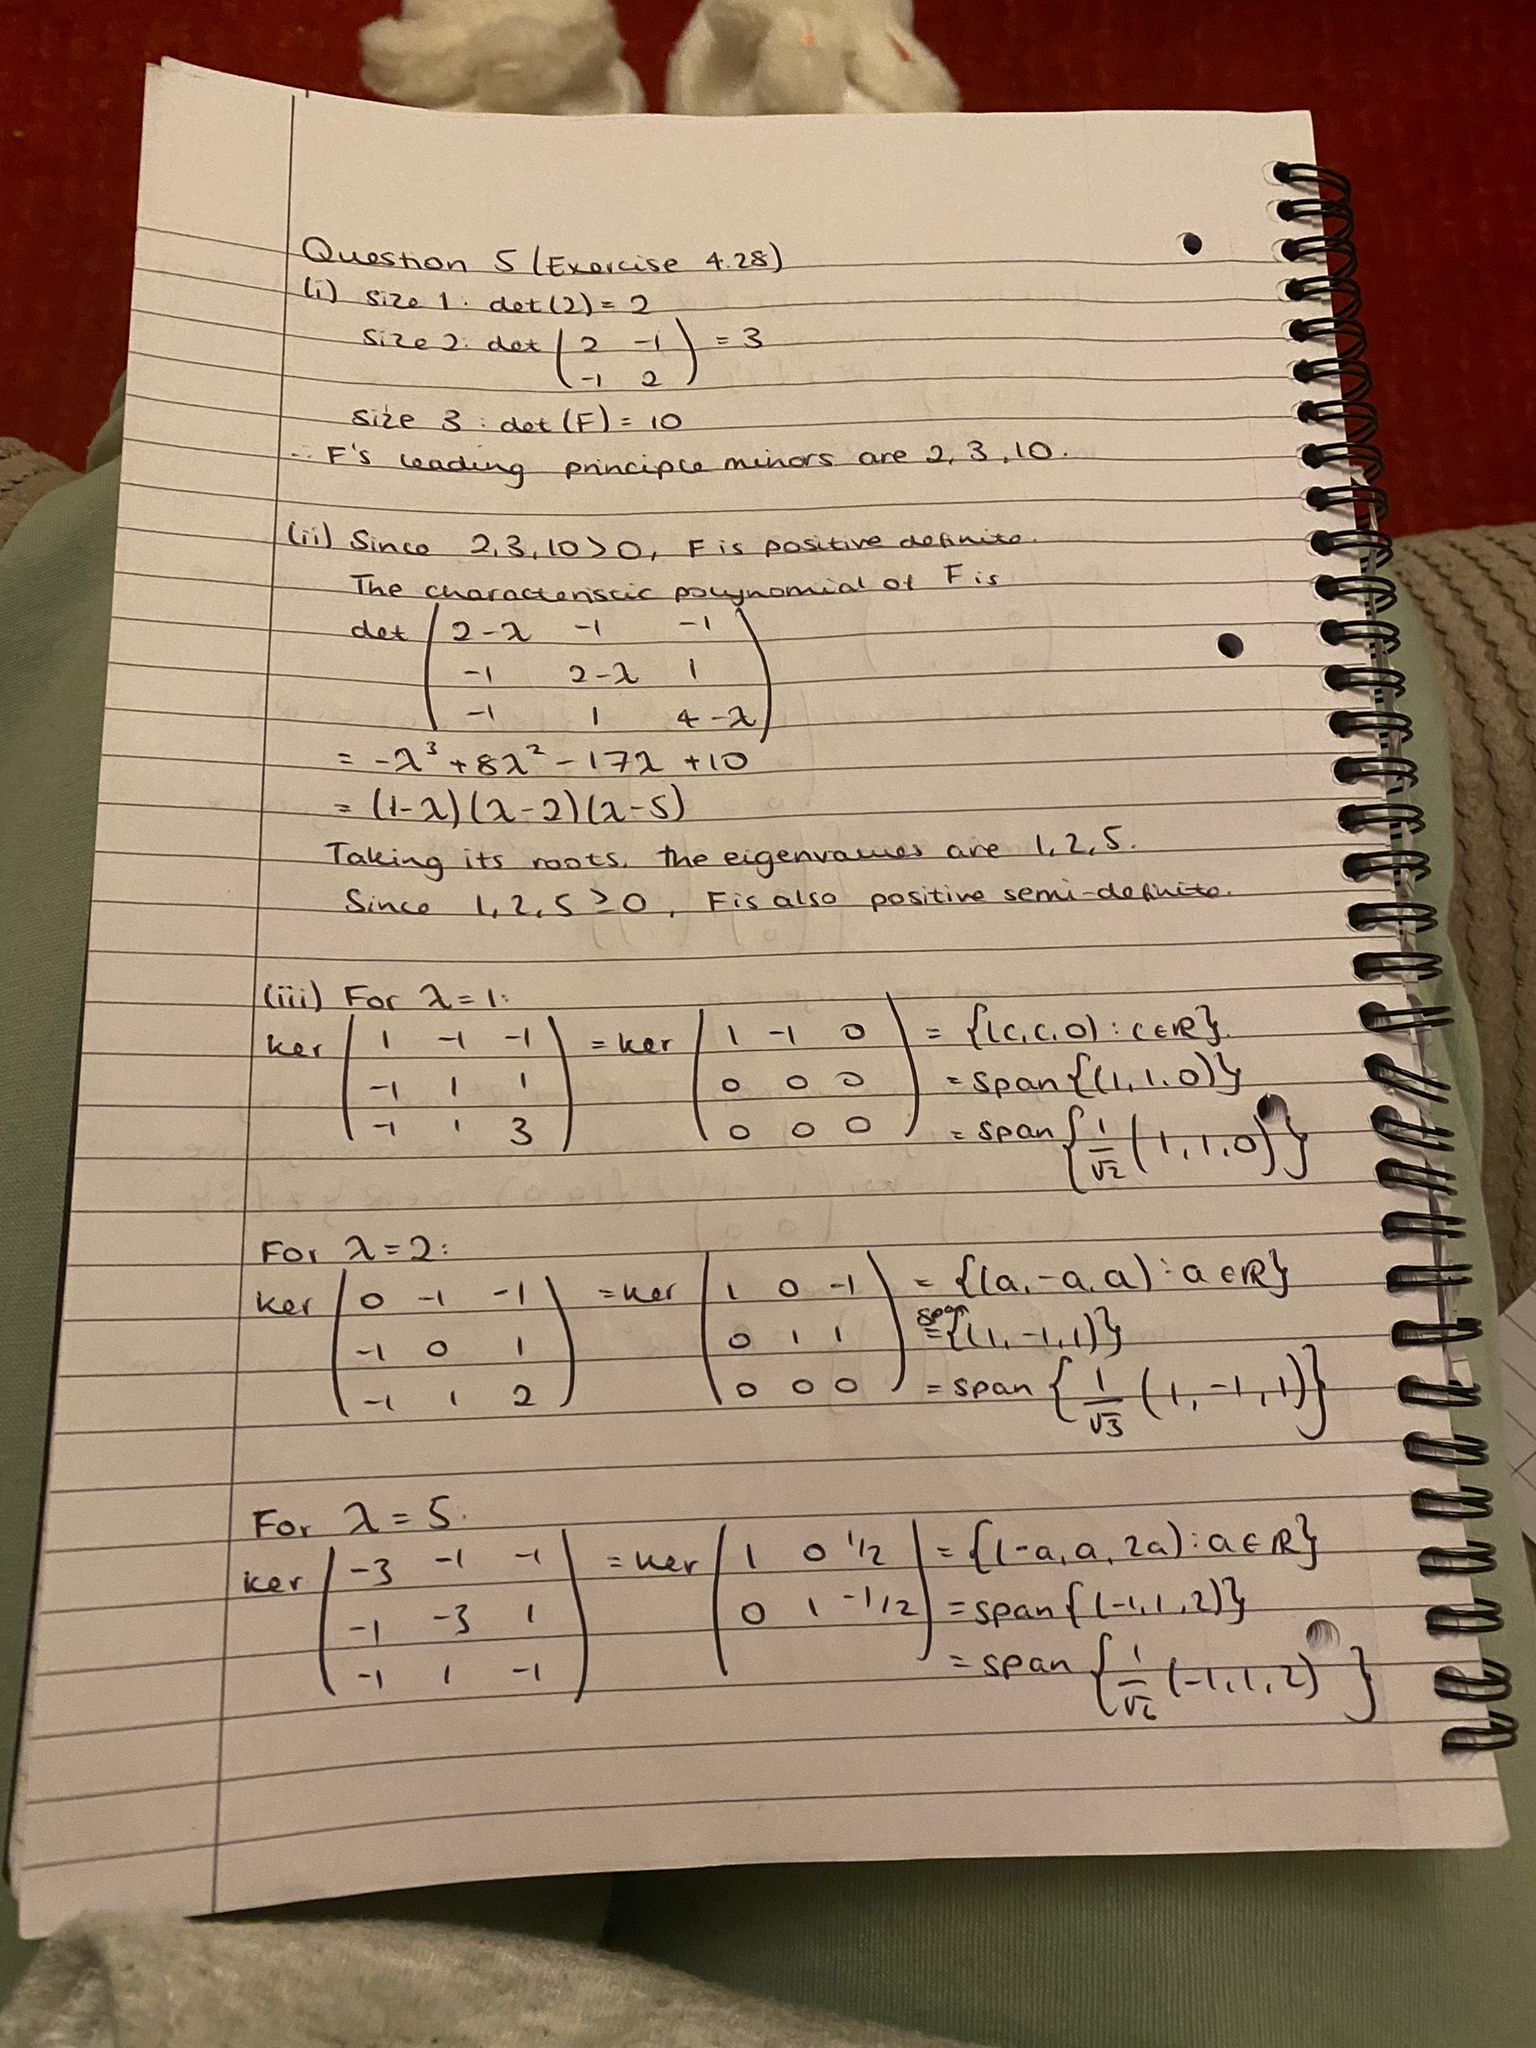
\includegraphics[scale = 0.2]{IMG-20231126-WA0003.jpg}


\includegraphics[scale = 0.25]{WhatsApp Image 2023-11-26 at 17.30.35_a5f8feeb.jpg}

\break
\section{Part C}
First the bilinear form on the Minkowski space is the interval of a "$3+1$" dimensional vector. The Minkowski space is a spacial case of the metric on a local space in general relativity \cite{Gravitation} which reduces to the theory of special relativity. In special relativity\cite{Special} the interval is an invariant under the Lorentz transform given conventionally by $ds^2 = c^2dt^2 - dx^2 - dy^2 - dz^2$. This can be expressed using the bilinear form.

\setlength{\belowdisplayskip}{0pt} \setlength{\belowdisplayshortskip}{0pt}
\setlength{\abovedisplayskip}{0pt} \setlength{\abovedisplayshortskip}{0pt}

\begin{equation*}
    ds^2
    = <v_1|v_2>
    :=
    \begin{bmatrix}
        cdt_1 & dx_1 & dy_1 & dz_1
    \end{bmatrix}
    \begin{bmatrix}
        1 & 0 & 0 & 0 \\
        0 & -1 & 0 & 0 \\
        0 & 0 & -1 & 0 \\
        0 & 0 & 0 & -1
    \end{bmatrix}
    \begin{bmatrix}
        cdt_2 \\ dx_2 \\ dy_2 \\ dz_2
    \end{bmatrix}
\end{equation*}

Here we use the $(+,-,-,-)$ convention, while some sources\cite{Mink} use the $(-,+,+,+)$ definition of the linear form which multiplies the matrix by $-1$.

\subsection*{Bilinear Forms are "Fundamentally Different"}
We see that the bilinear form on $\mathbb{R}^4$ is an inner product as its known the dot product is an inner product. Example 2.16 is also an inner product from the question. Exercise 2.49 is linear as matrix products are linear. Then, its symmetric and positive definite from the question so its an inner product.

However, the Minkowski space is not positive definite as for an event at time zero $ds^2 = <e|e> = - (dx^2+dy^2+dz^2)$. Which is negative meaning that the bilinear form is not positive definite so its not an inner product. In this way the Minkowski space is fundamentally different.

\subsection*{Matrices Of Inner Products Are "The Same"}
For vectors in $\mathbb{R}^4$ we have $, v \cdot w = <v|w> := v^T I_4 w$. 
In the basis of $M_2(\mathbb{R})$ where each $b_i$ basis has a $1$ in a single element we again get $tr([v][w]^T) = <v|w> = v^T I_4 w$.


Then choosing the polynomial basis $\{ 1,x,x^2,x^3 \}$ we have that $\int_0^1 [v](t)[w](t)\,dt = <v|w> = v^T \begin{bmatrix}
    0&1&2&3\\1&2&3&4\\2&3&4&5\\3&4&5&6
\end{bmatrix} w$ \cite{Wolf}. Then since the polynomial inner product matrix is symmetric we can use a change of basis to reduce it to a diagonal matrix by spectral decomposition theorem which is changed to the identity\cite{GTP}. Hence we see that for some basis all the spaces have the same inner product when expressed as a matrix and dimension so can be considered "the same".



\begin{thebibliography}{11}

\bibitem{Gravitation}
Misner, C. W., Thorne, K. S., \& Wheeler, J. A. (1973). Gravitation. Princeton University Press.

\bibitem{Special}
 Einstein, A. (1905) . On the electrodynamics of moving bodies. Annalen der Physik, 17(10), 891-921.

 \bibitem{Mink}
H. Minkowski. (1909). Space and Time. Physikalische Zeitschrift.

\bibitem{Wolf}
Wolfram Research. (2009). Wolfram Alpha. www.wolframalpha.com

\bibitem{GTP}
OpenAI. (2022). GPT-3.5. chat.openai.com/










\end{thebibliography}




\end{document}
